\documentclass[aspectratio=169,t]{beamer}
\usefonttheme[onlymath]{serif}
\usepackage[utf8]{inputenc}
\usepackage{graphicx}
\usepackage{subcaption}
\usepackage{color}
\usepackage{graphicx}
\usepackage{fancybox}
\usepackage[vlined]{algorithm2e}
\usepackage{anyfontsize}
\usepackage{standalone}
\usepackage{tikz}
\usetikzlibrary{shapes,arrows.meta}
\tikzset{%
	>={Latex[width=2mm,length=2mm]},
	%Colors
	blackStyle/.style = {draw=black, fill=lightgray},
	tealStyle/.style = {draw=MyTeal, fill=MyLtTeal},
	coralStyle/.style = {draw=MyCoral, fill=MyLtCoral},
	sandStyle/.style = {draw=MySand, fill=MyLtSand},
	%Base Styles
	base/.style = {
		draw=black, fill=white, thick,
		text centered, font=\sffamily, inner sep=.2cm},
	baseVar/.style = {base, rectangle, rounded corners,
		minimum width=1cm, minimum height=1cm},
	baseOp/.style = {base, ellipse,
		minimum width=1cm, minimum height=1cm,
		align=center},
	baseLine/.style = {thick},
	%Colored Styles
	algNode/.style = {baseOp, blackStyle},
	algLine/.style = {baseLine, draw=black},
	%
	givNode/.style = {baseVar, tealStyle},
	givLine/.style = {baseLine, draw=MyTeal},
	%
	genNode/.style = {baseVar, sandStyle},
	genLine/.style = {baseLine, draw=MySand},
	%
	outNode/.style = {baseVar, coralStyle},
	outLine/.style = {baseLine, draw=MyCoral},
}
\usepackage[acronym]{glossaries}
\makeglossaries

\usepackage{beamerthemesplit}
\usetheme[compress]{Heidelberg}
\definecolor{unirot}{rgb}{0.5976525,0,0}
\usecolortheme[named=unirot]{structure}

\title{Discrete Morse Theory}
\author{Bryan Wolfford}

\institute[Uni HD]{
	Universität Heidelberg\\
	Interdisciplinary Center for Scientific Computing\\
	Forensic Computational Geometry Laboratory\\
	\color{unirot}{wolfford@stud.uni-heidelberg.de}
}
\date{\today}

\begin{document}
%\input{myCommands.tex}
%\input{chapters/Z2-Glossary.tex}
\setlength{\intextsep}{0pt}
\def\hilite<#1>{\temporal<#1>{\color{black}}{\color{unirot}}{\color{gray}}}

\iffalse
\fi
%------------------------------------------------
\frame[plain]{
	\titlepage
}

%------------------------------------------------
\frame{\frametitle{Outline}
	%\tableofcontents[hideallsubsections]
	\begin{itemize}
		\item Motivation \& Introduction \pause
		\item Discrete Morse Theory
		%\begin{itemize}
		%	\item Mathematical Foundation
		%	\item Serial Algorithm
		%\end{itemize} \pause
		%\item Exploiting Parallelism
		%\begin{itemize}
		%	\item Basics
		%	\item Analysis of the Serial Algorithm
		%	\item Parallel Algorithm
		%\end{itemize} \pause
		%\item Experiments \& Evaluation
		%\begin{itemize}
		%	\item Filter Response on Synthetic and Acquired \tdd{}
		%	\item Performance of the Parallel Algorithm
		%\end{itemize} \pause
		\item Conclusions
	\end{itemize}
}




%================================================
%================================================
\section{Motivation \& Introduction}

%------------------------------------------------
\frame{\frametitle{Process Lower Stars - Voxel (1 of 2)}
	\begin{columns}[T]
		\begin{column}{.33\textwidth}
			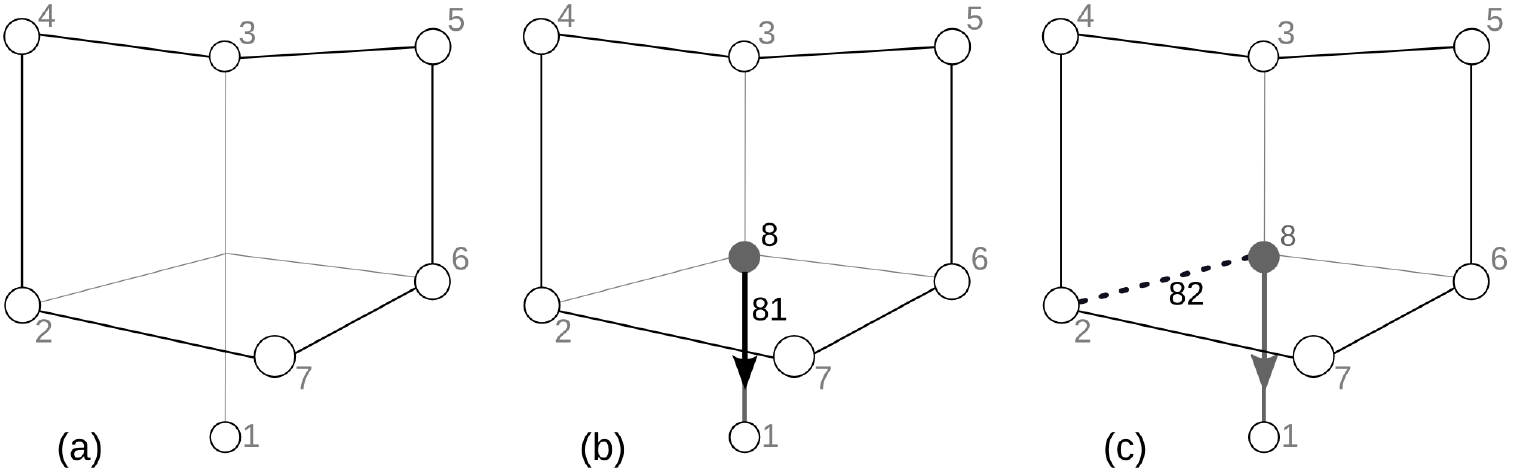
\includegraphics[width=\textwidth]{figures/gimp/processLowerStars_voxel_a.png}
		\end{column}
		\begin{column}{.33\textwidth}
			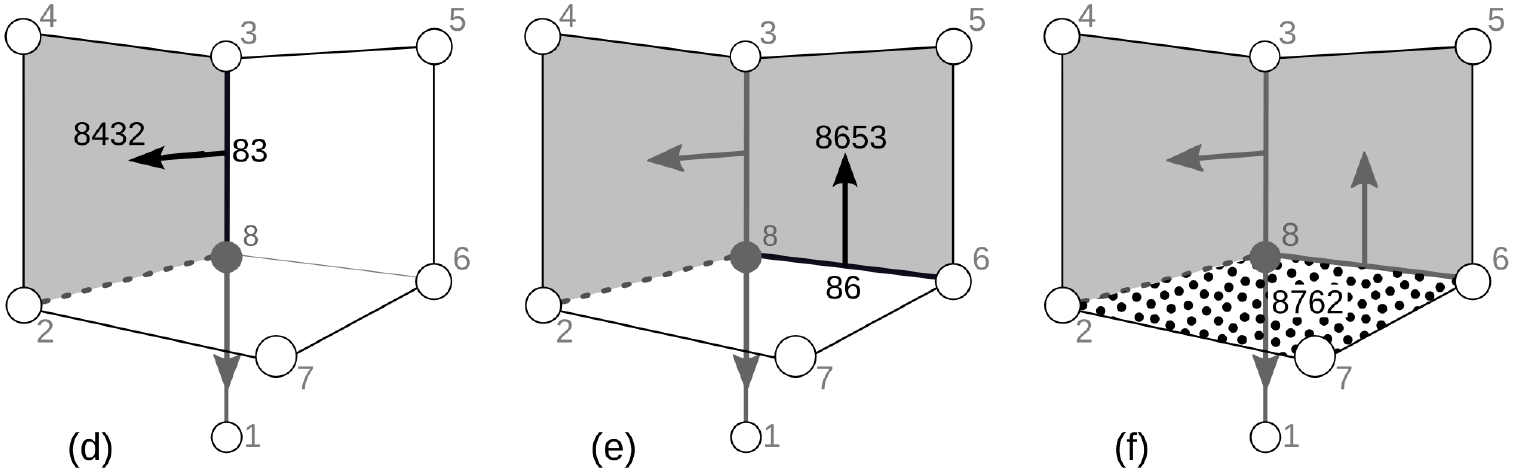
\includegraphics[width=\textwidth]{figures/gimp/processLowerStars_voxel_b.png}
		\end{column}
		\begin{column}{.33\textwidth}
			\includegraphics[width=\textwidth]{figures/gimp/processLowerStars_voxel_c.png}
		\end{column}
	\end{columns}
}

%------------------------------------------------
\frame{\frametitle{Process Lower Stars - Voxel (2 of 2)}
	\begin{columns}[T]
		\begin{column}{.33\textwidth}
			\includegraphics[width=\textwidth]{figures/gimp/processLowerStars_voxel_d.png}
		\end{column}
		\begin{column}{.33\textwidth}
			\includegraphics[width=\textwidth]{figures/gimp/processLowerStars_voxel_e.png}
		\end{column}
		\begin{column}{.33\textwidth}
			\includegraphics[width=\textwidth]{figures/gimp/processLowerStars_voxel_f.png}
		\end{column}
	\end{columns}
}

%------------------------------------------------
\frame{\frametitle{Sandstone ABCD}
	\begin{columns}[T]
		\begin{column}{\textwidth}
			\includegraphics[width=\textwidth]{figures/gimp/sandstone_abcd.png}
		\end{column}
	\end{columns}
}

%------------------------------------------------
\frame{\frametitle{Sandstone - Critical Cells}
	\begin{columns}[T]
		\begin{column}{.5\textwidth}
			\centering
			\includegraphics[width=.8\textwidth]{figures/gimp/sandstone_a.png}
		\end{column}
		\begin{column}{.5\textwidth}
			\centering
			\includegraphics[width=.8\textwidth]{figures/gimp/sandstone_b.png}
		\end{column}
	\end{columns}
}

%------------------------------------------------
\frame{\frametitle{Sandstone - Subsets}
	\begin{columns}[T]
		\begin{column}{.5\textwidth}
			\centering
			\includegraphics[width=.8\textwidth]{figures/gimp/sandstone_a.png}
		\end{column}
		\begin{column}{.25\textwidth}
			\includegraphics[width=\textwidth]{figures/gimp/sandstone_c.png}
		\end{column}
		\begin{column}{.2\textwidth}
			\includegraphics[width=\textwidth]{figures/gimp/sandstone_d.png}
		\end{column}
	\end{columns}
}

%------------------------------------------------
\frame{\frametitle{3D Foam}
	\begin{columns}[T]
		\begin{column}{.425\textwidth}
			\centering
			\includegraphics[width=\textwidth]{figures/gimp/foam.png}
		\end{column}
		\begin{column}{.575\textwidth}
			\begin{itemize}
				\item \hspace{1.75ex}262,144 voxels (64x64x64)
				\item 1,540,351 cells in the cubical complex
				\item \hspace{4ex}4,093 cells in the Morse complex
			\end{itemize}
		\end{column}
	\end{columns}
}
\end{document}
